\documentclass[utf8, xcolor=dvipsnames,ngerman]{beamer}
% \documentclass[utf8, xcolor=dvipsnames,english,handout]{beamer}

\usepackage{soul} 
\usepackage{pifont} 
\usepackage{pgfplots}
\usepackage{subcaption}
\usepackage[english]{babel}
\usepackage{pgf}
\usepackage{tikz}
\usetikzlibrary{shapes}
\usetikzlibrary{arrows,backgrounds,automata}
\usetikzlibrary{positioning,shapes,matrix,calc}
\usepackage{xspace}
\usepackage{pgfpages}
\usepackage{booktabs}
\usepackage{multirow}
\usepackage{diagbox}
\usepackage{graphicx}
\usepackage{hyperref}


% \pgfpagesuselayout{4 on 1}[a4paper,border shrink=5mm,landscape]

\setbeameroption{hide notes}
%\setbeameroption{show notes}
%\setbeameroption{show notes on second screen}
%\setbeameroption{show only notes}

\newcommand{\univ}{\ensuremath{\mathcal{X}}\xspace}

\mode<presentation> {
   \usecolortheme{seahorse}
   \usecolortheme{rose}

   \definecolor{tudo}{RGB}{18,102,172}
   \colorlet{tudodark}{tudo!70!black}%{tudo!55!black}
    \definecolor{nicebrown}{RGB}{219,179,143}

   \setbeamercolor{structure}{fg=tudodark}

   \usefonttheme[onlymath]{serif}

   \useinnertheme{rounded}
   \setbeamertemplate{items}[circle]
   \setbeamertemplate{blocks}[rounded][shadow=false]
   \setbeamertemplate{footline}
{
  \hfill%
  \usebeamercolor[fg]{page number in head/foot}%
  \usebeamerfont{page number in head/foot}%
  \insertframenumber\kern.5em\vskip2pt%
} 

}

\setbeamercolor{frametitle}{fg=tudodark}
\setbeamertemplate{frametitle}
{
\begin{centering}%
\insertframetitle\par\vspace{4pt}%
\color{tudodark} \hrule width \textwidth height 1pt%
\end{centering}%
}

\tikzset{onslide/.code args={<#1>#2}{%
  \only<#1>{\pgfkeysalso{#2}} % \pgfkeysalso doesn't change the path
}}
\newcommand{\putat}[3]{\begin{picture}(0,0)(0,0)\put(#1,#2){#3}\end{picture}}
\tikzset{onslide/.code args={<#1>#2}{%
  \only<#1>{\pgfkeysalso{#2}} % \pgfkeysalso doesn't change the path
}}
\tikzset{temporal/.code args={<#1>#2#3#4}{%
  \temporal<#1>{\pgfkeysalso{#2}}{\pgfkeysalso{#3}}{\pgfkeysalso{#4}} % \pgfkeysalso doesn't change the path
}}

\newenvironment<>{varblock}[2][.9\textwidth]{%
  \setlength{\textwidth}{#1}
  \begin{actionenv}#3%
    \def\insertblocktitle{#2}%
    \par%
    \usebeamertemplate{block begin}}
  {\par%
    \usebeamertemplate{block end}%
  \end{actionenv}}
  
\newenvironment<>{statusblock}[1]{%
  \begin{actionenv}#2%
      \def\insertblocktitle{#1}%
      \par%
      \mode<presentation>{%
%        \setbeamercolor{block title}{fg=white,bg=orange!20!black}
%        \setbeamercolor{block body}{fg=black,bg=olive!50}
       \setbeamercolor{block title}{bg=nicebrown!50,fg=black!70!nicebrown}
     }%
      \usebeamertemplate{block begin}}
    {\par\usebeamertemplate{block end}\end{actionenv}}

\setbeamertemplate{navigation symbols}{}

\newcommand{\paper}[1]{\begin{footnotesize}\color{tudodark}{[#1]}\end{footnotesize}}
\newcommand{\citep}[1]{\paper{#1}}

\newcommand{\cmark}{\ding{51}}%
\newcommand{\xmark}{\ding{55}}%
% \newcommand{\tp}[0]{\intercal}%
\newcommand{\tp}[0]{\top}%
\newcommand{\norm}[1]{\left\lVert#1\right\rVert}
\newcommand{\setST}{\ \middle|\ } % used to get a nice delimiter within \left\{...}\right; adaptive solution would be better
\newcommand{\win}[1]{$\hspace{-0.3mm}$\textbf{#1}}
\newcommand{\size}[1]{|#1|}
% \newcommand{\sizeV}[1]{|#1|^{\hspace{-.15em}\textit{\tiny V}}}
\newcommand{\sizeV}[1]{|#1|}
% \newcommand{\sizeE}[1]{|#1|_{\hspace{-.15em}\textit{\tiny E}}}
\newcommand{\sizeE}[1]{\left\lVert#1\right\rVert}
% \newcommand{\sizeVE}[1]{|#1|^{\hspace{-.15em}\textit{\tiny V}}_{\hspace{-.15em}\textit{\tiny E}}}
\newcommand{\attr}[0]{\alpha}
\newcommand{\lab}[0]{\tau}
\newcommand{\wag}[0]{\nabla_{\hspace{-.15em}w}}
\newcommand{\wdpg}[0]{\times_{\hspace{-.15em}w}}
\newcommand{\iso}[0]{\psi}
\newcommand{\comp}[1]{\overline{#1}}
% \newcommand{\splitcomp}[1]{{#1}^\complement}
\newcommand{\splitcomp}[1]{\widetilde{#1}}

% numbers
\newcommand{\bbR}[0]{\ensuremath{\mathbb{R}}\xspace}
\newcommand{\bbRnn}[0]{\ensuremath{\mathbb{R}_{\geq0}}\xspace}
\newcommand{\bbRp}[0]{\ensuremath{\mathbb{R}^+}\xspace}
\newcommand{\bbN}[0]{\ensuremath{\mathbb{N}}\xspace}
\newcommand{\bbNp}[0]{\ensuremath{\mathbb{N}^+}\xspace}

\newcommand{\bigO}[0]{\ensuremath{\mathcal{O}}}
\newcommand{\cNP}[0]{\ensuremath{\mathsf{NP}}}
\newcommand{\cP}[0]{\ensuremath{\mathsf{P}}}
\newcommand{\cGI}[0]{\ensuremath{\mathsf{GI}}\xspace}

\newcommand{\EdgeSet}[1]{\ensuremath{[#1]^2}}
\newcommand{\diEdgeSet}[1]{\ensuremath{#1 \times #1}}

\newcommand{\wlength}[0]{\ensuremath{\ell}}

\newcommand{\hilb}[0]{\ensuremath{\mathcal{H}}\xspace}
\newcommand{\graphs}[0]{\ensuremath{\mathcal{G}}\xspace}
\newcommand{\powset}[0]{\ensuremath{\mathcal{P}}\xspace}
% \newcommand{\powset}[0]{\ensuremath{\mathfrak{P}}\xspace}
\newcommand{\linegraph}[1]{\ensuremath{L(#1)}\xspace}
\newcommand{\subdivgraph}[1]{\ensuremath{S(#1)}\xspace}


%% global vector style
\let\vec\mathbf


%% additional functions
\DeclareMathOperator{\N}{N}
\DeclareMathOperator{\Aut}{Aut}
\DeclareMathOperator{\dom}{dom}
\DeclareMathOperator{\codom}{codom}
\DeclareMathOperator{\img}{img}
\DeclareMathOperator{\csi}{cisi}
\DeclareMathOperator{\sm}{sm}
\DeclareMathOperator{\enc}{enc}
\DeclareMathOperator{\ip}{i}
\DeclareMathOperator{\s}{s}
\DeclareMathOperator{\p}{p}
\DeclareMathOperator{\feat}{feat}
\DeclareMathOperator{\dist}{dist}
\DeclareMathOperator{\tr}{tr}
\DeclareMathOperator{\RBF}{RBF}
\DeclareMathOperator{\DPG}{DPG}
\DeclareMathOperator{\poly}{poly}
\DeclareMathOperator{\bin}{bin}
\DeclareMathOperator{\BS}{bs}
\DeclareMathOperator{\WSKR}{wskr}
\DeclareMathOperator{\FV}{fv}
\DeclareMathOperator{\CAN}{CAN}

\DeclareMathOperator{\id}{id}
\DeclareMathOperator{\type}{type}
% argmax and argmin
\DeclareMathOperator*{\argmax}{arg\,max}
\DeclareMathOperator*{\argmin}{arg\,min}

%% common subgraph 
\DeclareMathOperator{\childB}{childB}
\DeclareMathOperator{\childS}{childS}
\DeclareMathOperator{\parentS}{parentS}
\DeclareMathOperator{\REF}{ref}
\DeclareMathOperator{\tw}{tw}
\DeclareMathOperator{\NTD}{NTD}
\DeclareMathOperator{\NTDG}{NTDG}
\newcommand{\MCSfunc}[3]{\ensuremath{\textsc{#1}(#2,#3)}}
\newcommand{\MCS}[2]{\MCSfunc{Mcs}{#1}{#2}}
% \newcommand{\MCCIS}[2]{\MCSfunc{Mccis}{#1}{#2}}
% \newcommand{\BBPMCCES}[2]{\MCSfunc{Bbp-Mcces}{#1}{#2}}
\newcommand{\MCCIS}[2]{\MCS{#1}{#2}}
\newcommand{\BBPMCCES}[2]{\MCS{#1}{#2}}
\newcommand{\sizeGraph}[1]{\ensuremath{\llbracket#1\rrbracket}}
\newcommand{\sMCS}[2]{\ensuremath{\sizeGraph{\MCS{#1}{#2}}}}
\renewcommand{\cmark}{\color{tudodark}{\ding{51}}}%
\renewcommand{\xmark}{\color{red}{\ding{55}}}%
\newcommand{\X}{\ensuremath{\chi}\xspace}
\newcommand{\Assign}{\ensuremath{\mathfrak{B}}\xspace}


% \newcommand{\paper}[1]{\begin{footnotesize}\color{tudodark}{{[#1]}}\end{footnotesize}}
% \newcommand{\citep}[1]{\paper{#1}}


\graphicspath{{figures/}}


\title{\textsc{TUDataset}: A collection of benchmark datasets for learning with graphs}
\author{%
Christopher Morris\inst{1} \and
\textbf{Nils M.~Kriege}\inst{2} \and
Franka Bause\inst{3} \and 
Kristian Kersting\inst{4} \and
Petra Mutzel\inst{5} \and
Marion Neumann\inst{6}
}
\institute{%
\inst{1} Polytechnique Montréal \and %
\inst{2} University of Vienna \and %
\inst{3} TU Dortmund University \and %
\inst{4} TU Darmstadt \and %
\inst{5} University of Bonn \and %
\inst{6} Washington University in St.~Louis %
}
                      
\date{July 17, 2020}


% \icmlaffiliation{darm}{}
% \icmlaffiliation{bonn}{}
% \icmlaffiliation{wustl}{}


\begin{document}
% For every picture that defines or uses external nodes, you'll have to
% apply the 'remember picture' style. To avoid some typing, we'll apply
% the style to all pictures.
\tikzstyle{every picture}+=[remember picture]

% By default all math in TikZ nodes are set in inline mode. Change this to
% displaystyle so that we don't get small fractions.
\everymath{\displaystyle}

\begin{frame}
 \titlepage
%  \putat{135}{-15}{
\includegraphics[height=1.6cm]{Uni_Logo_2016.pdf}}
\end{frame}


\begin{frame}{Graph Classification and Regression}

\begin{block}{Setting}
 \begin{description}
  \item[Input: ] Trainingset $T = \{(G_1,y_1),\dots,(G_n,y_n)\}$ of \textbf{graphs} $g_i \in \mathcal{G}$
and labels $y_i \in \mathcal{Y}$, $i \in \{1,2, \dots, n\}$.
  \item[Goal: ] Learn function $f : \mathcal{G} \to \mathcal{Y}$.
 \end{description} 
\end{block}

\begin{exampleblock}{}
\begin{columns}[c]
  \column{0.5\textwidth} 
    \begin{itemize}
      \item $\mathcal{G}$ -- set of molecules
      \item $\mathcal{Y} = \{\texttt{toxic}, \texttt{non-toxic}\}$
      \item $T$ -- tested molecules
    \end{itemize}
  \column{0.4\textwidth}
    \LARGE$f\left(\vcenter{\hbox{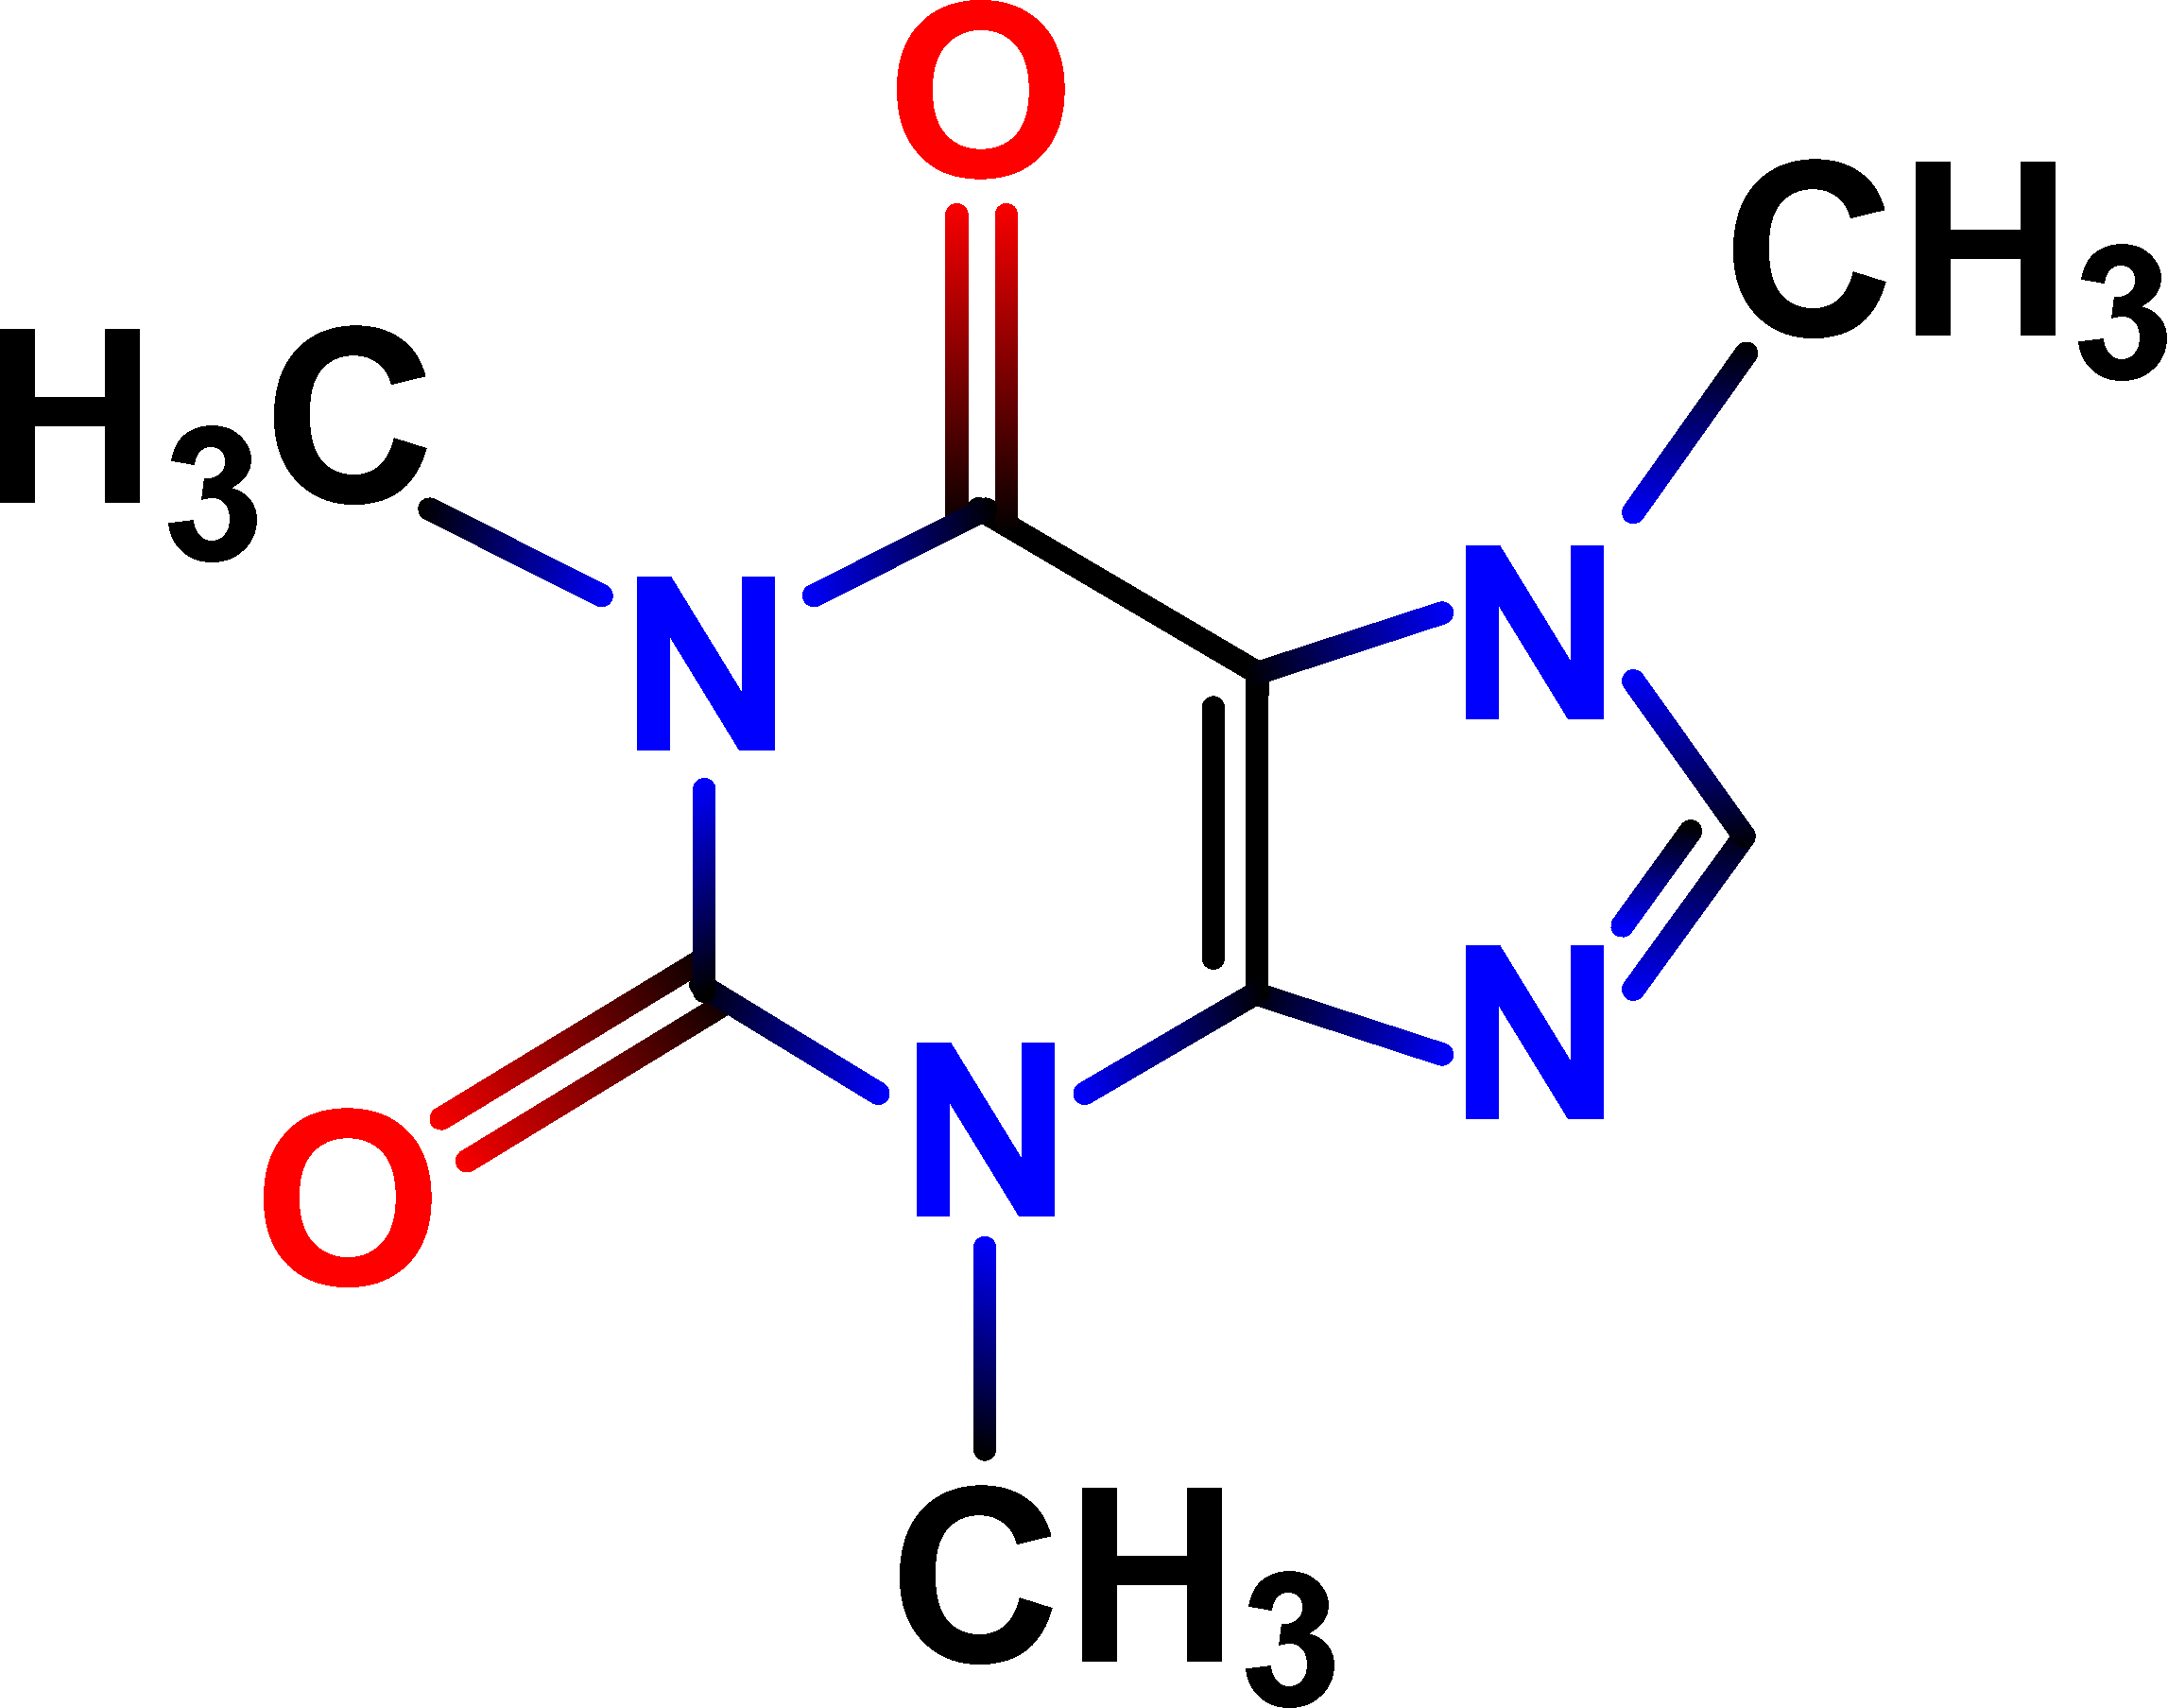
\includegraphics[width=1.9cm]{caffeine.pdf}}}\right)= \text{?}$
\end{columns}

\end{exampleblock}


\textbf{Approaches:}\\
\begin{itemize}
 \item Graph embedding, e.g., chemical fingerprints (1973)
 \item Graph kernels (2002)
 \item Graph neural networks (2016)
\end{itemize}
\end{frame}


\begin{frame}{Authoritative Experimental Evaluation}

\begin{block}{Problems}
 \begin{itemize}
  \item Graph models are non standardized 
  \item Experimental setup is not standardized
  \item[$\Rightarrow$] comparison of results from different publications not possible
  \item Missing comparison with baseline methods
  \item Used benchmark data sets are often 
  \begin{itemize}
    \item too small
    \item too easy to solve 
    \item insufficiently diverse
  \end{itemize}
 \end{itemize}
\end{block}
 
\end{frame}

\begin{frame}[t]{\textsc{TUDataset}: Contribution}

\begin{block}{(1) Datasets}
 \begin{itemize}
  \item \alert<2>{Small molecules}
  \item \alert<3>{Bioinformatics}
  \item \alert<4>{Computer vision}
  \item \alert<5>{Social networks}
  \item \alert<6>{Synthetic}
 \end{itemize}
\end{block}

\begin{center}
\only<2>{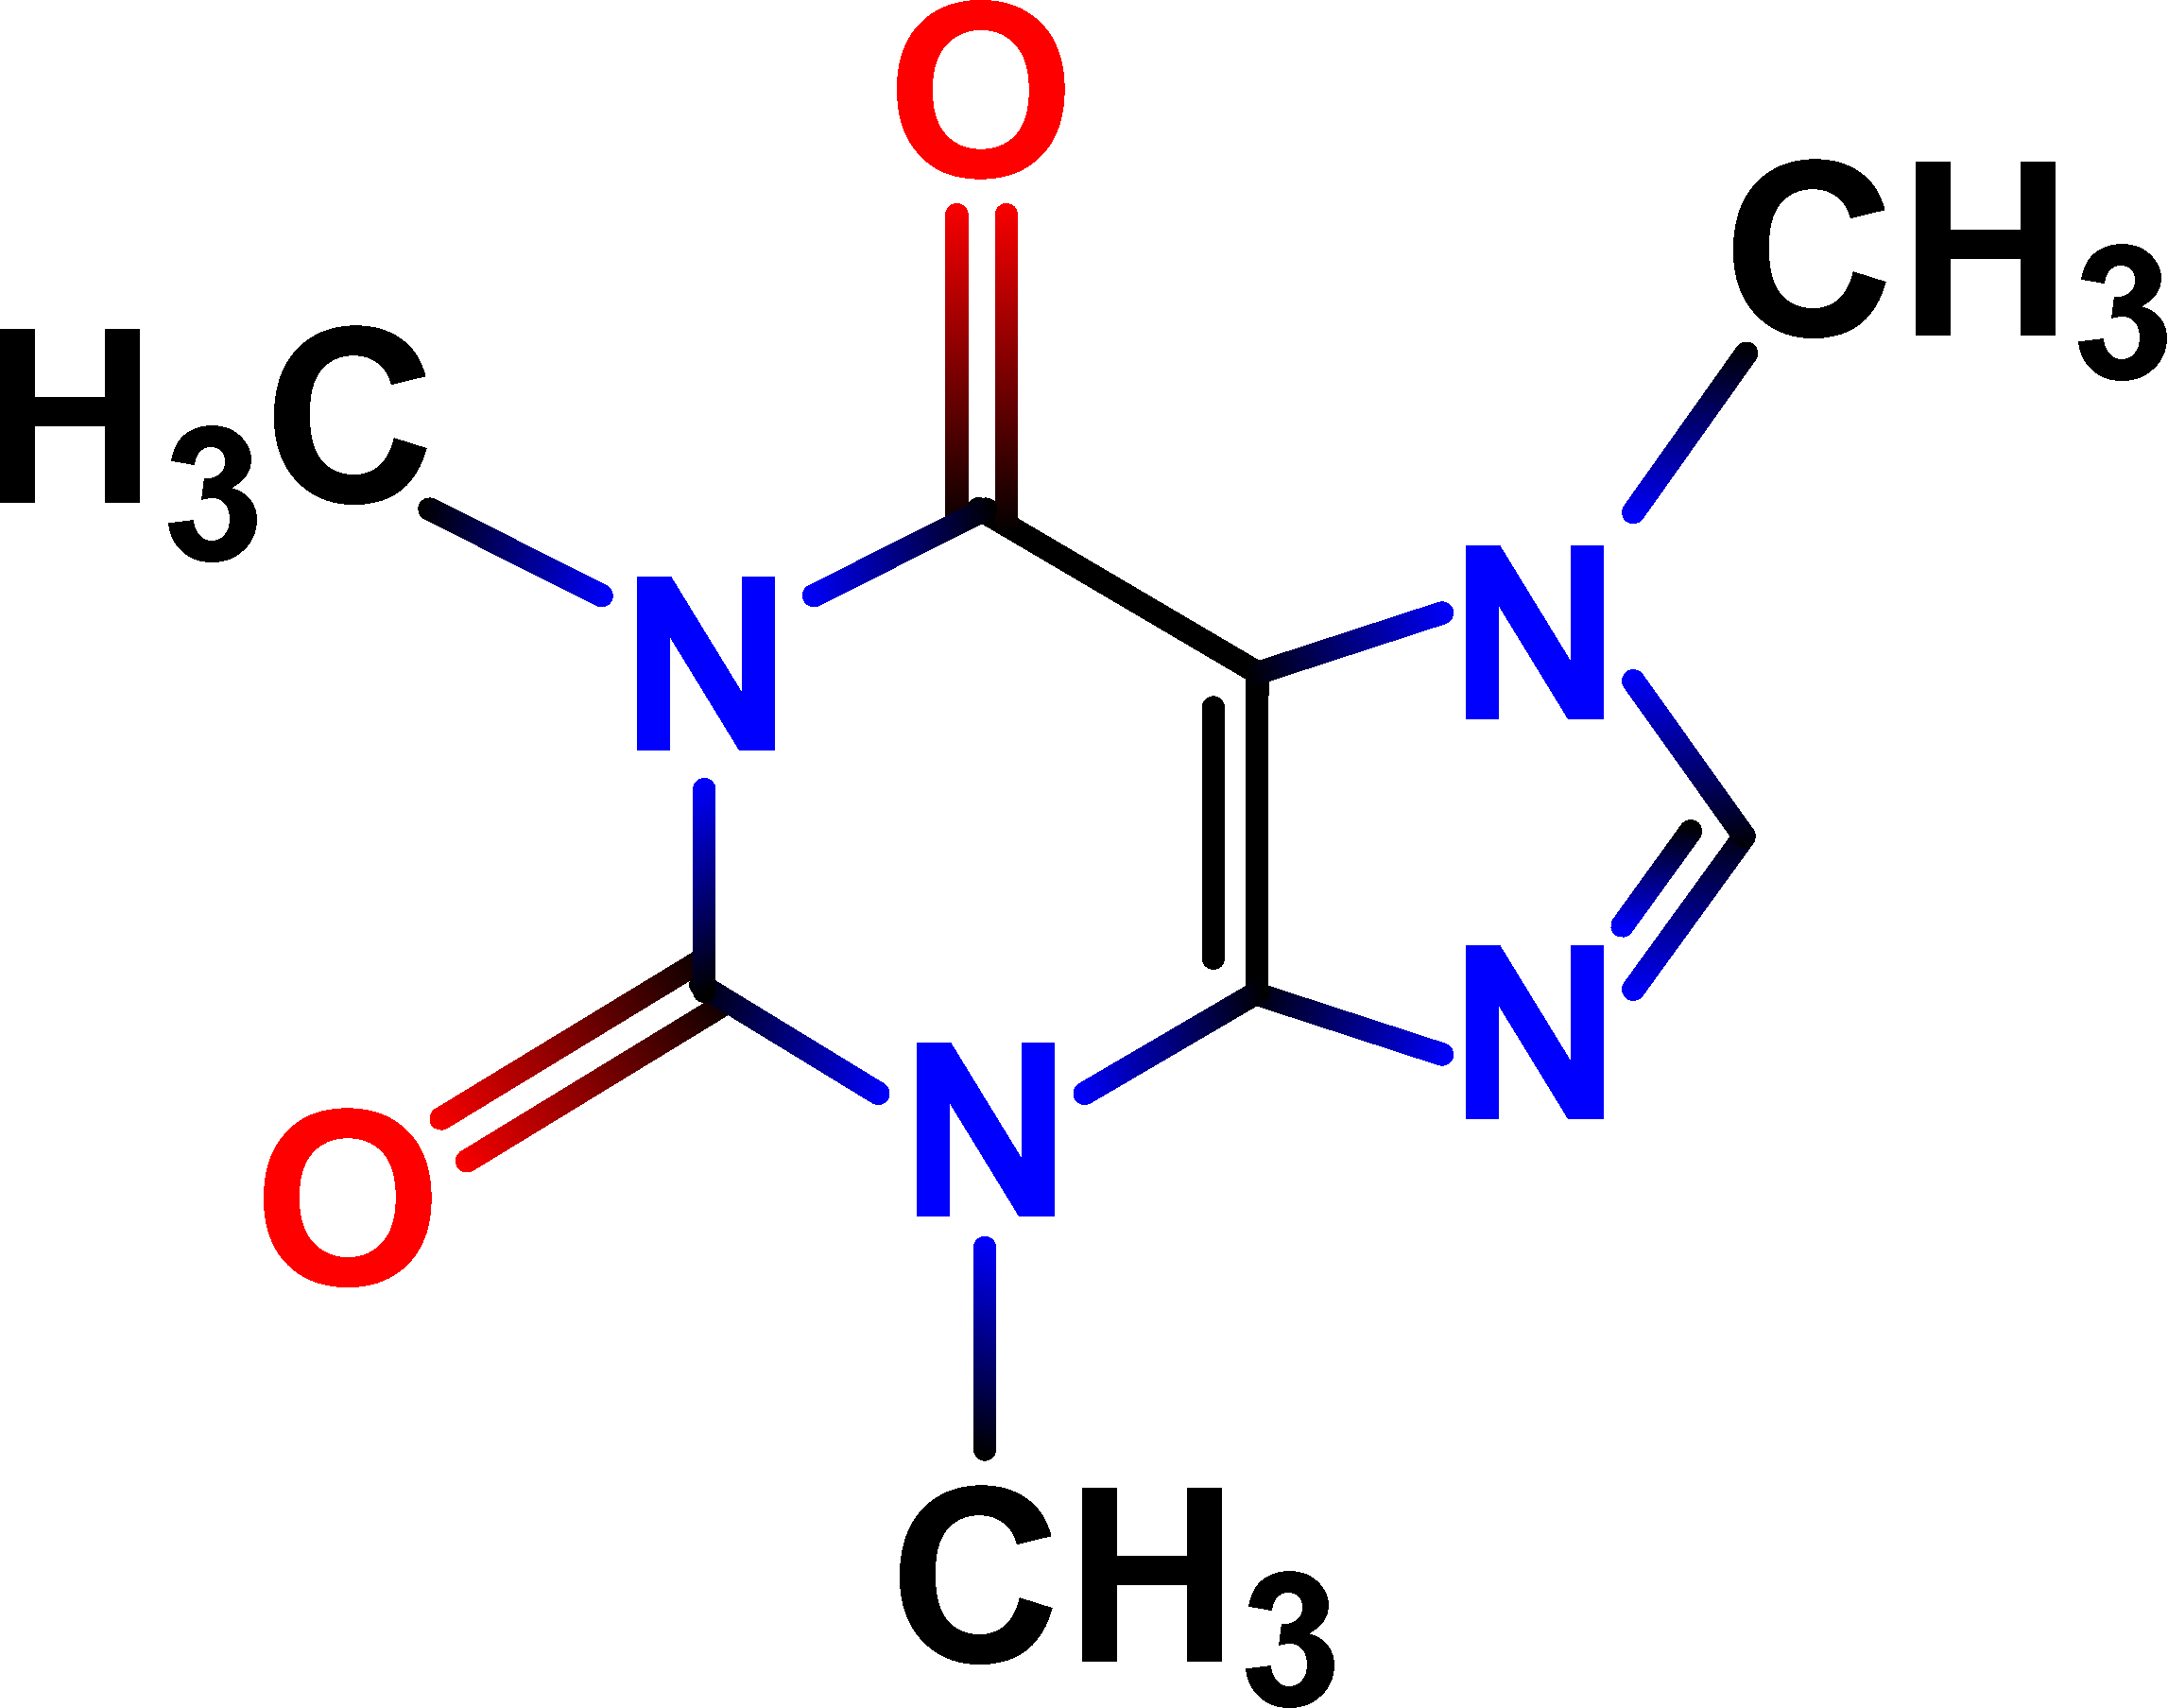
\includegraphics[height=3.5cm]{caffeine} \qquad 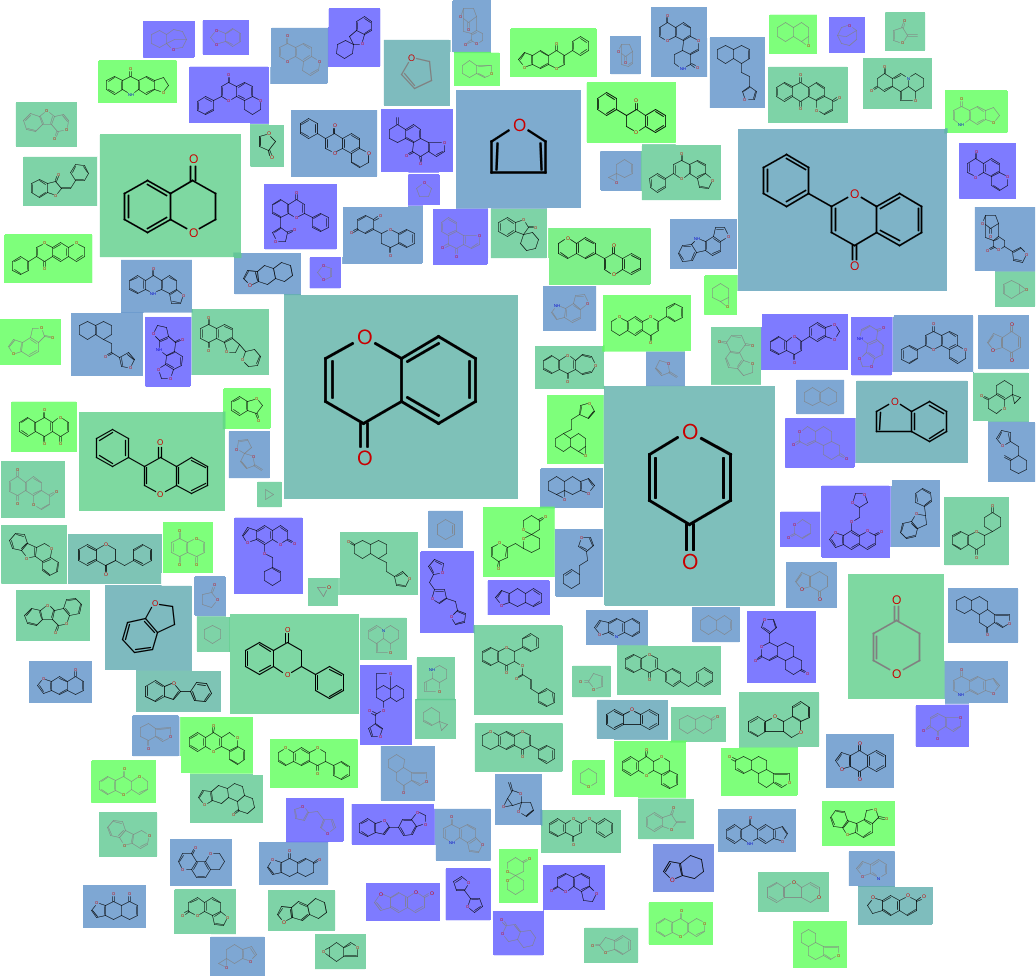
\includegraphics[height=3.5cm]{molecule_cloud.png}}%
\only<3>{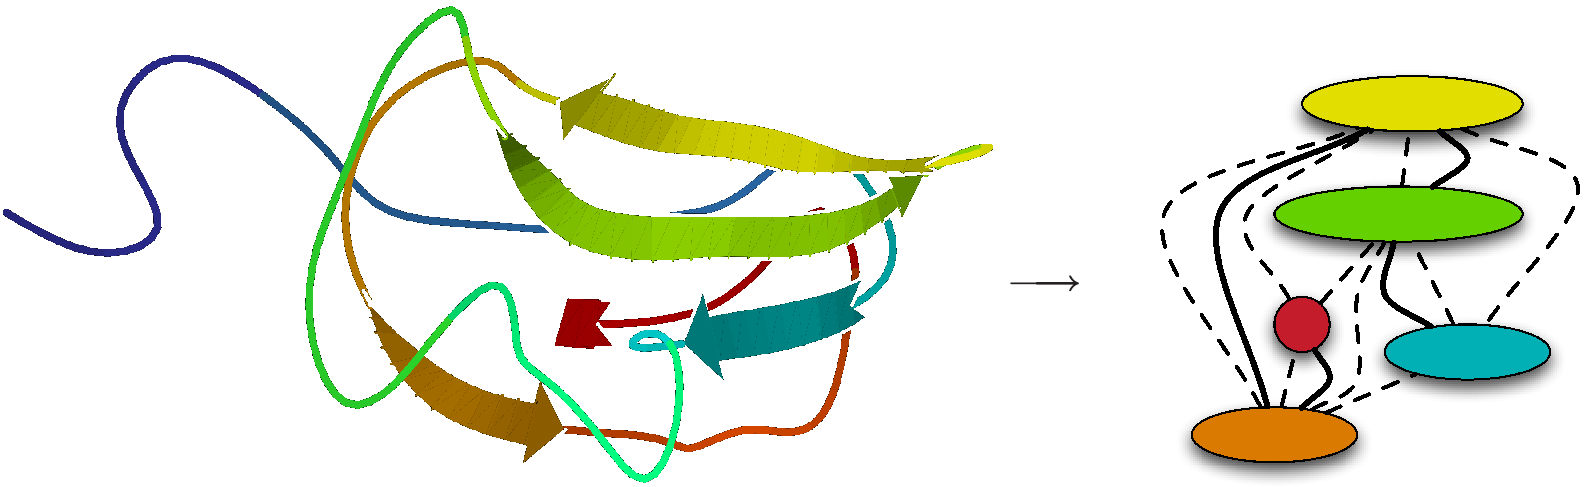
\includegraphics[height=3.1cm]{protein-graph}\\\hfill\paper{Borgwardt et al., 2005; Vishwanathan et al., 2010}}%
\only<4>{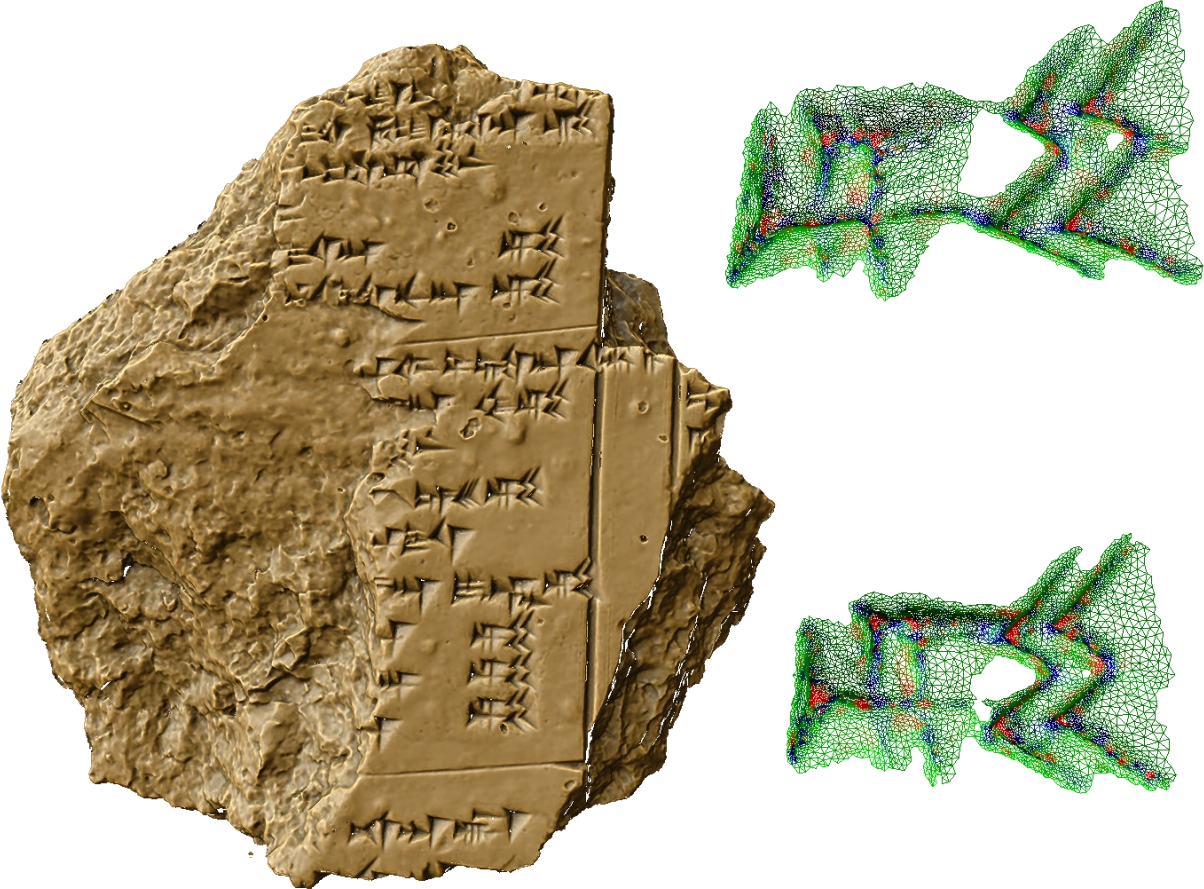
\includegraphics[height=3.1cm]{keil.png} \qquad 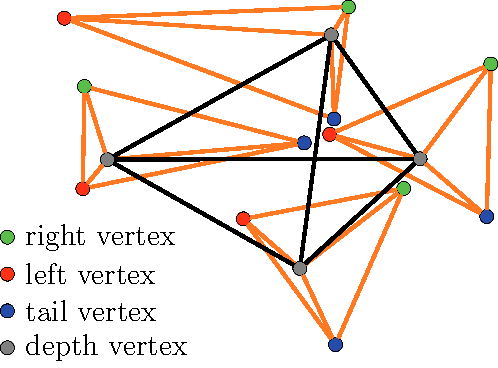
\includegraphics[height=3.1cm]{graph.pdf}\\\hfill\paper{Kriege et al., 2018}}%
\only<5>{%

\includegraphics[height=1cm]{IMDB_Logo_2016.pdf}\qquad

\includegraphics[height=.7cm]{GitHub_logo_2013.pdf}\qquad 

\includegraphics[height=1cm]{Twitter_bird_logo_2012.pdf}\\ \vspace{.7em}

\includegraphics[height=1cm]{Reddit_logo_new.pdf}\qquad

\includegraphics[height=1cm]{DBLP_Logo_320x120.png}\qquad

\includegraphics[height=1.1cm]{Facebook_f_logo.pdf}\\ \vspace{.7em}

\includegraphics[height=.9cm]{Deezer_logo.pdf}\qquad

\includegraphics[height=.9cm]{Twitch_logo_2019.pdf}
}%

\end{center}


\end{frame}


\begin{frame}{\textsc{TUDataset}: Our Contribution}

\begin{block}{(2) Baseline methods}
 \begin{itemize}
  \item Shortest-path kernel \paper{Borgwardt, Kriegel,2005}
  \item Graphlet \paper{Shervashidze et al., 2009} 
  \item Weisfeiler-Lehman subtree kernel \paper{Shervashidze et al., 2011}
  \item Weisfeiler-Lehman optimal assignment kernel \paper{Kriege et al., 2016}
  \item GNN architectures of PyTorch Geometric \paper{Fey, Lenssen, 2019}
 \end{itemize}
\end{block}

\pause

\begin{block}{(3) Evaluation Module}
 \begin{itemize}
  \item 10-fold cross validation
  \item Hyperparameter optimization for each fold
 \end{itemize}
\end{block}
 
\end{frame}


\begin{frame}{Summary}

\begin{itemize}
 \item Collection of over 120 graph datasets 
 \item Standard file format with data loaders
 \item Evaluation modules in Python
 \item Graph kernel baselines in C\texttt{++} with Python bindings
 \item Accessible via graph learning frameworks
\end{itemize}

\vspace{1.5em}

\pause

\begin{center}
 \Large{ \url{http://graphlearning.io}}
\end{center}

\vspace{1.5em}

\pause
\begin{block}{Thank You!}
\begin{itemize}
 \item Many thanks to all contributors of datasets
 \item Your contribution is highly welcome!
\end{itemize}

\end{block}



\end{frame}



\end{document}
